%% Document Class
\documentclass[a4paper]{article}

%% Language and font encodings
\usepackage[english]{babel}
\usepackage[utf8]{inputenc}
\usepackage[T1]{fontenc}
\usepackage{textcomp}
\usepackage[section]{placeins}
\usepackage{graphicx}
\usepackage{caption}
\usepackage{subcaption}
\usepackage{csquotes}
\usepackage{color,soul}
\usepackage{verbatim}

%% Sets page size and margins
\usepackage[a4paper,top=3cm,bottom=2cm,left=3cm,right=3cm,marginparwidth=2cm]{geometry}

%% Useful packages
\usepackage{amsmath}
\usepackage{amssymb}
\usepackage{graphicx}
\usepackage[colorinlistoftodos]{todonotes}
\usepackage[colorlinks=true, allcolors=blue]{hyperref}
\usepackage{multirow}
\usepackage[style=ieee]{biblatex}
\usepackage{filecontents}
\usepackage{listings}

%% Code Stuff
\usepackage{xcolor}
\usepackage{listings}
\definecolor{vgreen}{RGB}{104,180,104}
\definecolor{vblue}{RGB}{49,49,255}
\definecolor{vorange}{RGB}{255,143,102}
\lstdefinestyle{verilog-style} {
    language=Verilog,
    basicstyle=\small\ttfamily,
    keywordstyle=\color{vblue},
    identifierstyle=\color{black},
    commentstyle=\color{vgreen},
    numbers=left,
    numberstyle=\tiny\color{black},
    numbersep=10pt,
    tabsize=3,
    moredelim=*[s][\colorIndex]{[}{]},
    literate=*{:}{:}1 }

\makeatletter
\newcommand*\@lbracket{[}
\newcommand*\@rbracket{]}
\newcommand*\@colon{:}
\newcommand*\colorIndex{%
    \edef\@temp{\the\lst@token}%
    \ifx\@temp\@lbracket \color{black}%
    \else\ifx\@temp\@rbracket \color{black}%
    \else\ifx\@temp\@colon \color{black}%
    \else \color{vorange}%
    \fi\fi\fi
}
\newcommand*{\NumDoFiles}{5}%
\newcommand*{\NumSVFiles}{5}%
\def\app@exe{\immediate\write18}
\def\listDir#1#2{%
  \app@exe{ls #1/* | xargs cat >> files.tmp}%
  \lstinputlisting[#2]{files.tmp}%
  \AtEndDocument{}}

  \def\listAllFilesWithName#1#2{%
    \app@exe{ls #1 | xargs cat >> ./wow.tmp}%
    \lstinputlisting[#2]{./wow.tmp}%
    \AtEndDocument{rm -f ./wow.tmp}}

\makeatother
\usepackage{pgffor}%


%%Bibliography
\begin{filecontents}{references.bib}
@online{book,
  author = {"David Harris, Sarah Harris"},
  title = {"Digital Design and Computer Architecture"},
  year = {2012},
  journal = {Elsevier Science & Technology},
  howpublished = {"ProQuest Ebook Central, \url{http://ebookcentral.proquest.com/lib/osu/detail.action?docID=980017}"}}

@misc{dennard, title={IBM’s DRAM inventor Bob Dennard gets chip industry’s highest honor}, url={https://venturebeat.com/2019/11/07/ibms-dram-inventor-bob-dennard-gets-chip-industrys-highest-honor/}, publisher={Venture Business}, author={Takahashi, Dean}, year={2019}, month={November}}

@misc{fujio, title={Unsung Hero}, url={https://www.forbes.com/global/2002/0624/030.html#1406a92a3da3}, publisher={Forbes}, author={Fulford, Benjamin}, year={2002}, month={June}}
\end{filecontents}
\addbibresource{references.bib}



\begin{document}



\begin{titlepage}
 \begin{center}
  \vspace*{3cm}

  \large\textbf{ECE 271}

  \vspace{2cm}

  \huge\textbf{Digital Logic Design\\Final Project}

  \vspace{.5cm}

  \large\textbf{Nick Olson\\Michael ASD\\Sienna ASD}

  \vfill

  \normalsize November 30, 2019\\
  Instructor Shuman\\
  Oregon State University

  \vspace{0.8cm}
 \end{center}
\end{titlepage}



\tableofcontents
\listoffigures



\clearpage



\section{Project Description}
Intro to Project paragraph. The inputs and outputs of the overall design immediately follow. An overall description diagram is then shown in \textbf{Figure 1} and a hardware diagram is shown in \textbf{Figure 2}.

\begin{itemize}
  \item \textbf{Inputs:  } inputs
  \item \textbf{Outputs: } outputs
\end{itemize}

\begin{figure}[h]
  \centering
  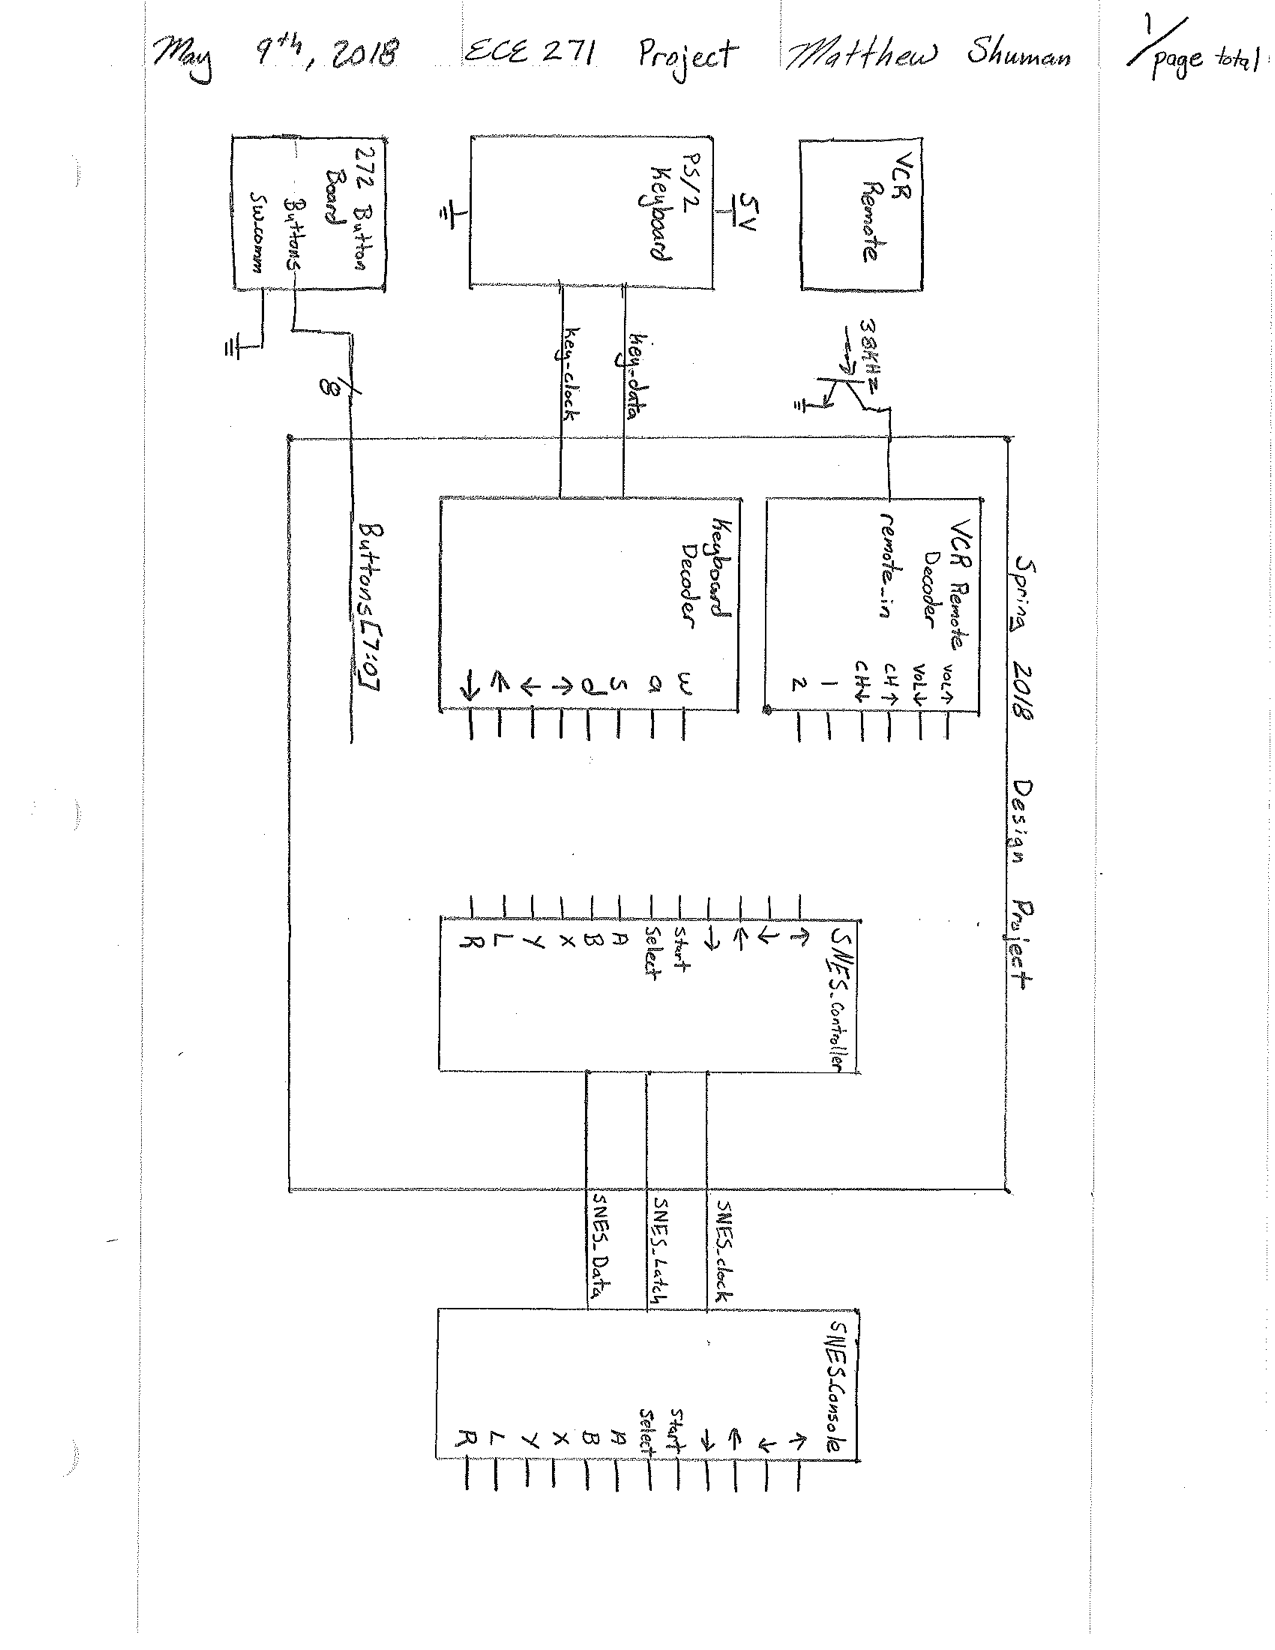
\includegraphics[width=.8\textwidth]{images/description.png}
	\caption{This image is legible, and conveys the point of the design.  Your image can be hand drawn, but it must have straight lines, use your OSU ID.  I don't recommend drafting this on the computer, because there aren't any decent tools to draw these block diagrams quickly.}
  \label{fig:description}
\end{figure}

\begin{figure}[h]
  \centering
    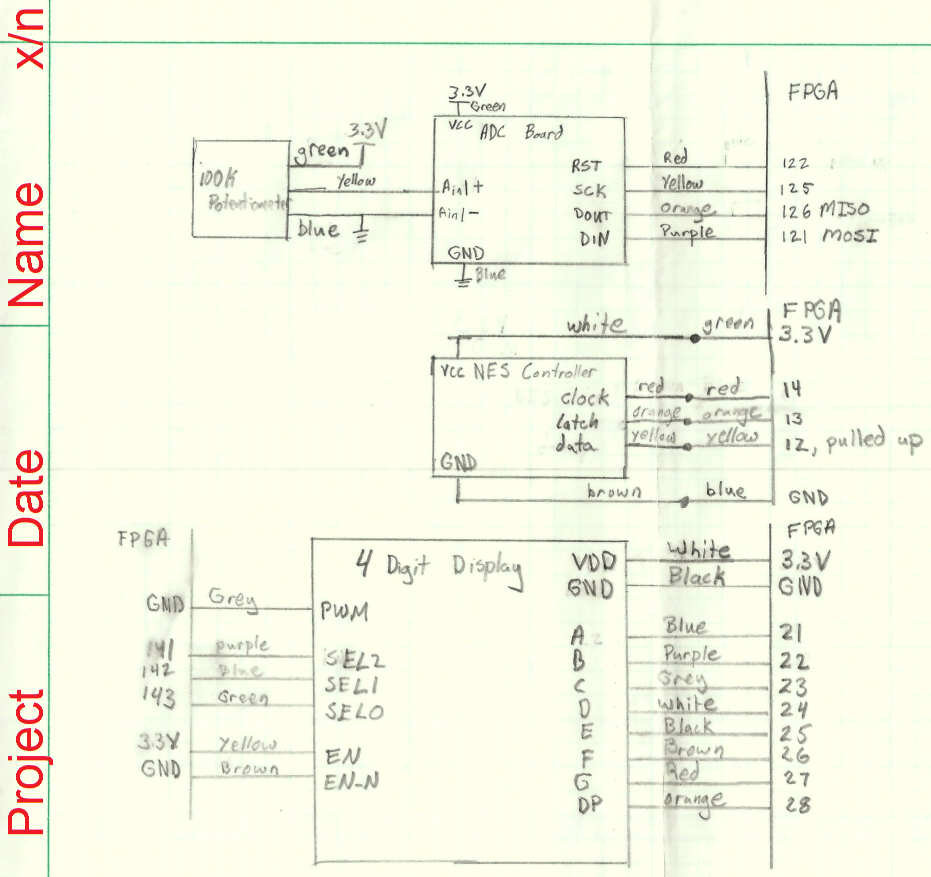
\includegraphics[width=.8\textwidth]{images/hardware.png}
	\caption{The hardware diagram shows which pins are used on the FPGA, module boards, and relevant supply voltages for the different pieces of hardware used in the system.}
    \label{fig:hardware}
\end{figure}



\clearpage



\section{High Level Description}
Top level introduction. The input and output specifications follow, a toplevel diagram follows in \textbf{Figure 3}, and the simulation results follow in \textbf{Figure 4}.
\begin{itemize}
  \item \textbf{Inputs:  } inputs
  \item \textbf{Outputs: } outputs
\end{itemize}
\begin{figure}[h]
  \centering
    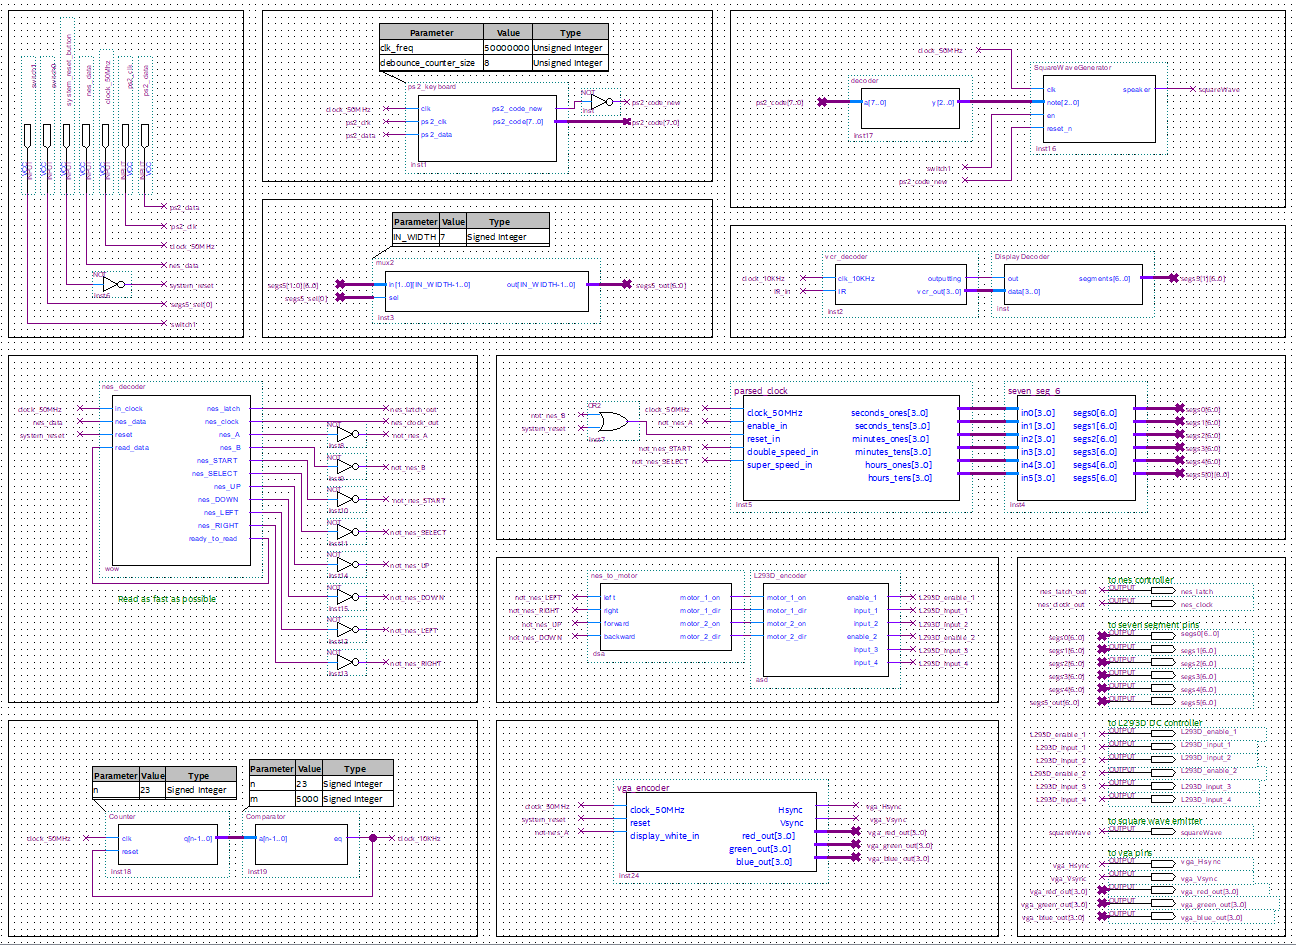
\includegraphics[width=.8\textwidth]{images/top_level.png}
	\caption{The top level design for the  project.  This would be improved by combining the priority encoder and Mux4 into a single clock select block.  Combining the ArrowLogic and Counter14 would also make this diagram better.  Use chapter 1 concepts wisely on this diagram, specifically hierarchy, modularity, regularity, and discipline.}
    \label{fig:top-level}
\end{figure}
\begin{figure}[h]
  \centering
    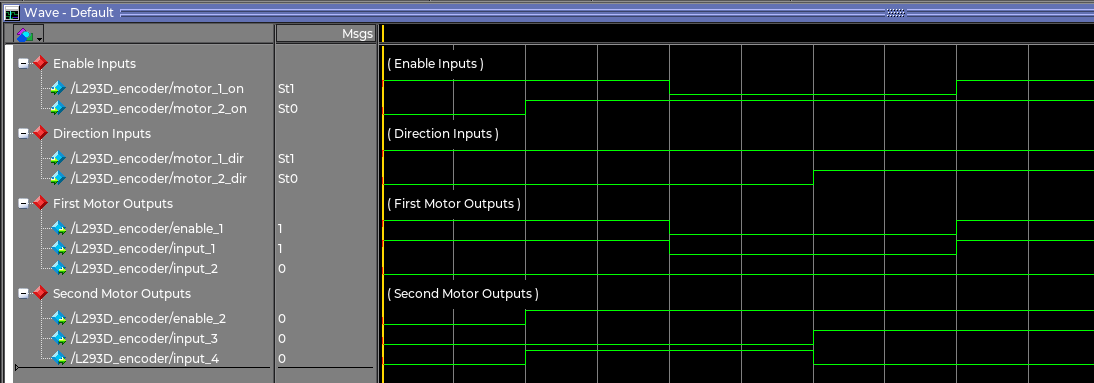
\includegraphics[width=.98\textwidth]{sims/top_level.png}
	\caption{The simulation results of the top level design for the  project.}
    \label{fig:top-level-sim}
\end{figure}
The following subsections will discuss the inputs, outputs, designs, and simulation results of all elements of the design at two levels of scrutiny: functional units and individual blocks of digital logic.



\clearpage



\subsection{Functional Unit 1 Name}
Introduction to functional unit. The input and output specifications follow, a block diagram of the unit follows in \textbf{Figure A}, the simulation results for the unit follows in \textbf{Figure B}, and the details for each individual block comprising the unit follow after.
\begin{itemize}
  \item \textbf{Inputs:  } inputs
  \item \textbf{Outputs: } outputs
\end{itemize}
\begin{figure}[h]
  \centering
    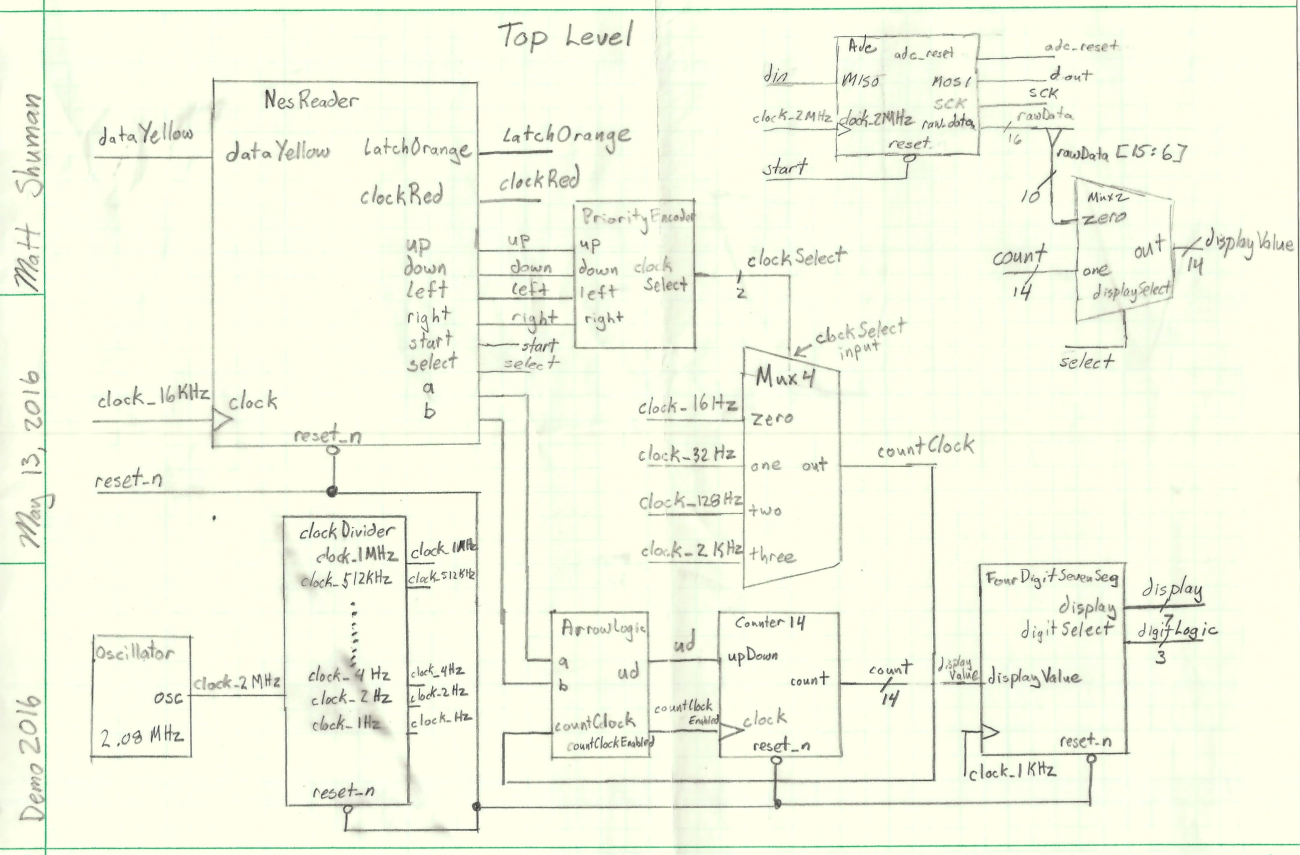
\includegraphics[width=.8\textwidth]{images/functional_1.png}
	\caption{The logic design of the (NAME) functional unit used in the final design.}
    \label{fig:functional-1}
\end{figure}
\begin{figure}[h]
  \centering
    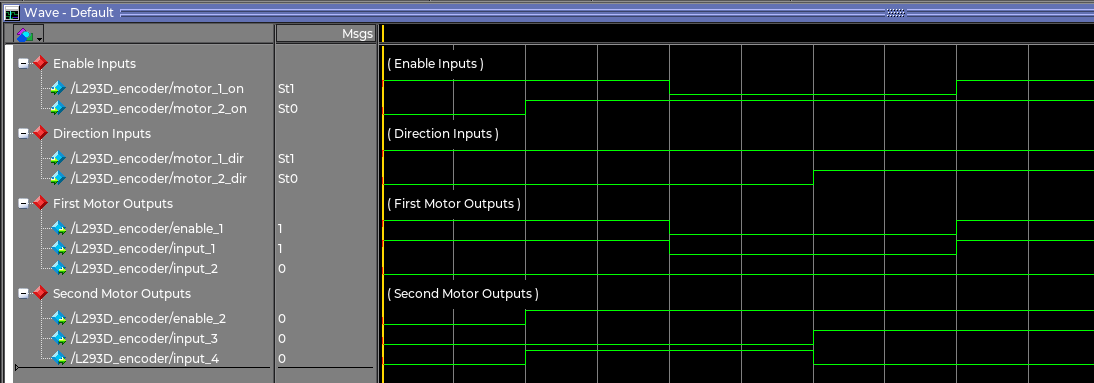
\includegraphics[width=.98\textwidth]{sims/functional_1.png}
	\caption{The simulation results of the top level design for the project.}
    \label{fig:top-level-sim}
\end{figure}



\clearpage



\subsubsection{Individual Block 1 Name (with testbench)}
Introduction to individual block. The input and output specifications follow, as well as the block diagram (\textbf{Figure C}), and simulation results \textbf{Figure D} for the individual block.
\begin{itemize}
  \item \textbf{Inputs:  } inputs
  \item \textbf{Outputs: } outputs
\end{itemize}
\begin{figure}[h]
  \centering
  \begin{subfigure}[t]{.4\textwidth}
    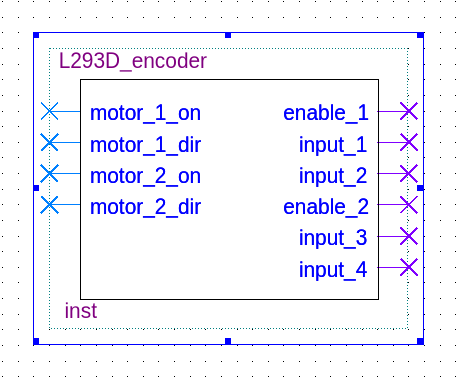
\includegraphics[width=.98\textwidth]{symbols/individual_placeholder.png}
    \subcaption{The block symbol of the (NAME) individual block used in the (NAME) functional unit.}
	\end{subfigure}
  \begin{subfigure}[t]{.4\textwidth}
  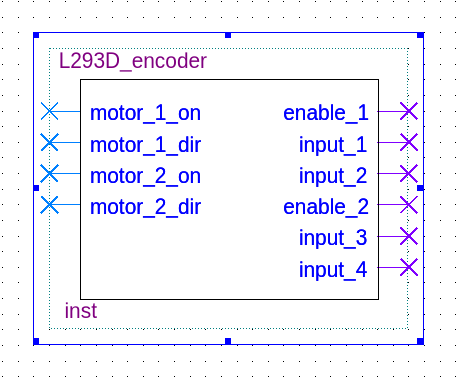
\includegraphics[width=.98\textwidth]{symbols/individual_placeholder.png}
  \subcaption{The block symbol of the test block used in the testbench made to further simulate the (NAME) individual block.}
  \end{subfigure}
  \centering
  \begin{subfigure}[t]{.98\textwidth}
    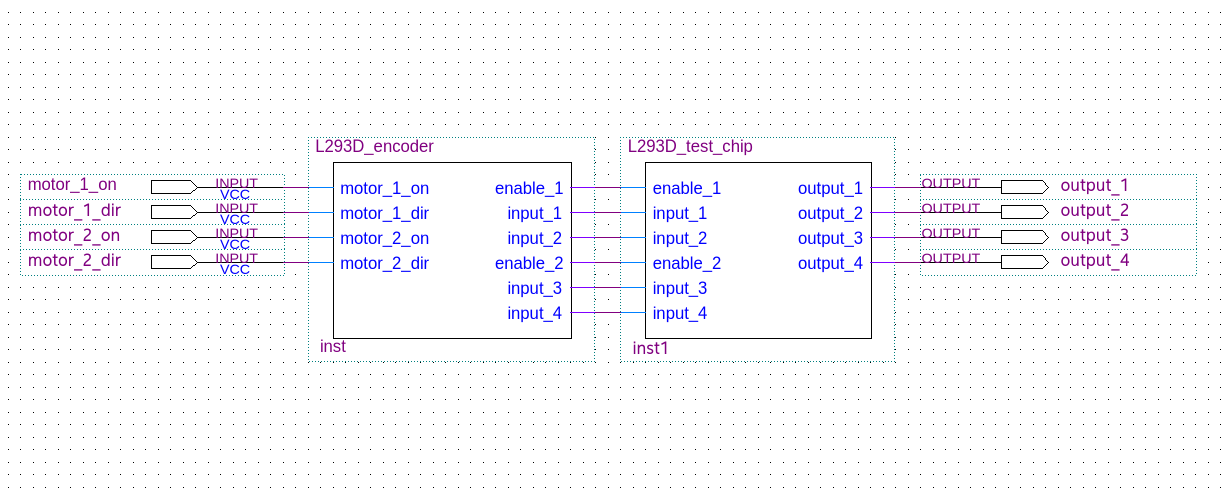
\includegraphics[width=.98\textwidth]{images/testbench_placeholder.png}
    \subcaption{The testbench used to further simulate the (NAME) individual block.}
  \end{subfigure}
  \caption{The block symbol of the (NAME) individual block used in the (NAME) functional unit, the block diagram of the logic of the testbench used to further simulate the block, and the block symbol of the test chip used in the testbench of the block.}
    \label{fig:individual-1-1-block}
\end{figure}
\begin{figure}[h]
  \centering
  \begin{subfigure}[t]{.98\textwidth}
    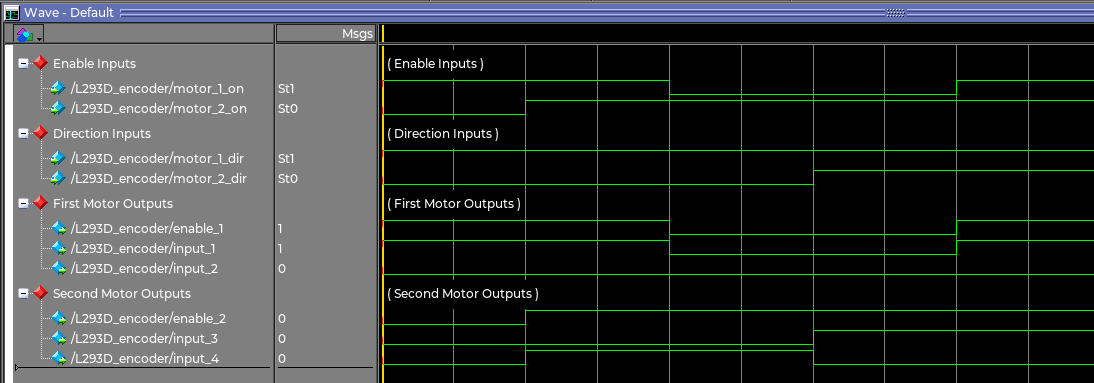
\includegraphics[width=.98\textwidth]{sims/placeholder_sim.png}
    \subcaption{The simulation results for the (NAME) individual block alone.}
  \end{subfigure}
  \begin{subfigure}[t]{.98\textwidth}
    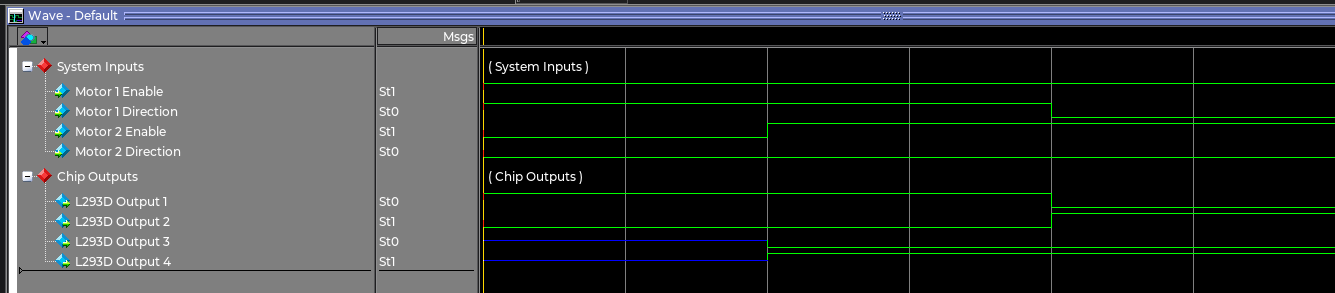
\includegraphics[width=.98\textwidth]{sims/placeholder_testbench_sim.png}
    \caption{The simulation results of the test block used in the testbench.}
  \end{subfigure}
  \begin{subfigure}[t]{.98\textwidth}
    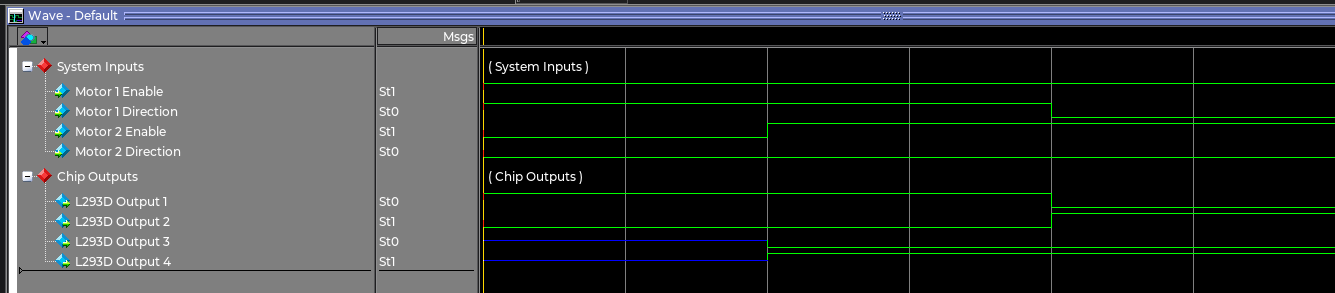
\includegraphics[width=.98\textwidth]{sims/placeholder_testbench_sim.png}
    \caption{The simulation results of the testbench used.}
  \end{subfigure}
    \caption{The simulation results of the block alone, the testbench used to further simulate the block, and the simulation results for the testbebch of the (NAME) individual block used in the (NAME) functional unit.}
    \label{fig:individual-1-1-sim}
\end{figure}



\clearpage



\subsubsection{Individual Block 2 Name (without testbench)}
Introduction to individual block. The input and output specifications follow, as well as the block diagram (\textbf{Figure C}), and simulation results \textbf{Figure D} for the individual block.
\begin{itemize}
  \item \textbf{Inputs:  } inputs
  \item \textbf{Outputs: } outputs
\end{itemize}
\begin{figure}[h]
  \centering
  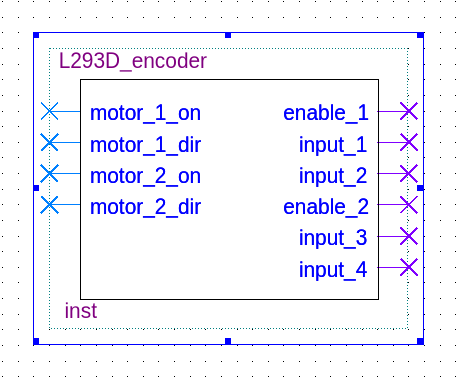
\includegraphics[width=.48\textwidth]{symbols/individual_placeholder.png}
  \caption{The block symbol of the (NAME) individual block used in the (NAME) functional unit.}
    \label{fig:individual-1-2-block}
\end{figure}
\begin{figure}[h]
  \centering
  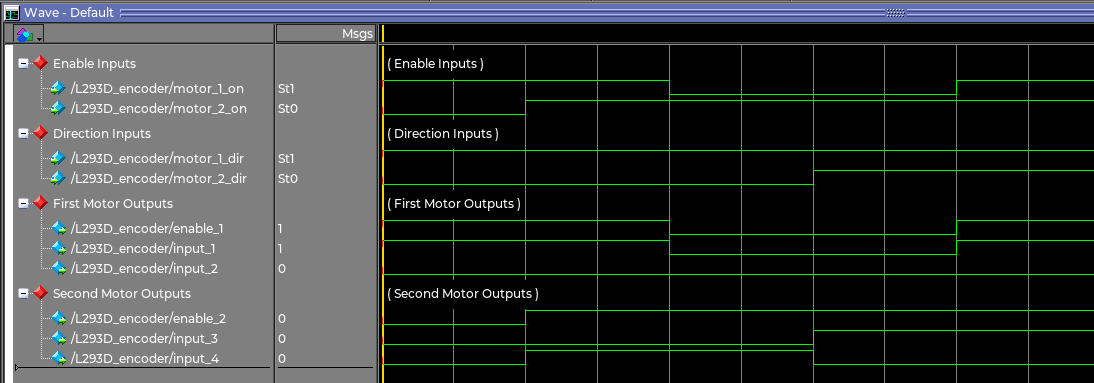
\includegraphics[width=.98\textwidth]{sims/placeholder_sim.png}
  \caption{The simulation results of the (NAME) individual block used in the (NAME) functional unit.}
    \label{fig:individual-1-2-sim}
\end{figure}



\clearpage



\appendix
\section{SystemVerilog Files}
This appendix will list the SystemVerilog code used for each block used in the design project.

\subsection{Functional Unit Name}
\begin{figure}[h]
  \lstinputlisting[style=verilog-style]{sv_files/placeholder.sv}
  \subcaption{SystemVerilog code for the (NAME) block used in the design.}
\end{figure}
\begin{figure}[h]
  \lstinputlisting[style=verilog-style]{sv_files/placeholder.sv}
  \subcaption{SystemVerilog code for the (NAME) block used in the design.}
\end{figure}
\begin{figure}[h]
  \lstinputlisting[style=verilog-style]{sv_files/placeholder.sv}
  \subcaption{SystemVerilog code for the (NAME) block used in the design.}
\end{figure}



\clearpage



\subsection{Functional Unit Name}
\begin{figure}[h]
  \lstinputlisting[style=verilog-style]{sv_files/placeholder.sv}
  \subcaption{SystemVerilog code for the (NAME) block used in the design.}
\end{figure}
\begin{figure}[h]
  \lstinputlisting[style=verilog-style]{sv_files/placeholder.sv}
  \subcaption{SystemVerilog code for the (NAME) block used in the design.}
\end{figure}
\begin{figure}[h]
  \lstinputlisting[style=verilog-style]{sv_files/placeholder.sv}
  \subcaption{SystemVerilog code for the (NAME) block used in the design.}
\end{figure}



\clearpage



\section{Simulation Files (Do Scripts)}
This appendix will list the Do Scripts used to simulate each block used in the design project.


\foreach \c in {1,2,...,\NumDoFiles}{%
    \IfFileExists{./do_files/\c_*.do} {%
        wow
        % \listAllFilesWithName{./do_files/\c_*.do}{}
    }{%
            % files does not exist, so nothing to do
    }%
}%




% \listDir{./do_files}{style=verilog-style}

\subsection{Functional Unit Name}
\begin{figure}[h]
  \lstinputlisting[style=verilog-style]{sv_files/placeholder.sv}
  \subcaption{Do Script for the (NAME) block used in the design.}
\end{figure}
\begin{figure}[h]
  \lstinputlisting[style=verilog-style]{sv_files/placeholder.sv}
  \subcaption{Do Script code for the (NAME) block used in the design.}
\end{figure}
\begin{figure}[h]
  \lstinputlisting[style=verilog-style]{sv_files/placeholder.sv}
  \subcaption{Do Script code for the (NAME) block used in the design.}
\end{figure}



\clearpage



\subsection{Functional Unit Name}
\begin{figure}[h]
  \lstinputlisting[style=verilog-style]{sv_files/placeholder.sv}
  \subcaption{Do Script for the (NAME) block used in the design.}
\end{figure}
\begin{figure}[h]
  \lstinputlisting[style=verilog-style]{sv_files/placeholder.sv}
  \subcaption{Do Script code for the (NAME) block used in the design.}
\end{figure}
\begin{figure}[h]
  \lstinputlisting[style=verilog-style]{sv_files/placeholder.sv}
  \subcaption{Do Script code for the (NAME) block used in the design.}
\end{figure}


\end{document}
